%!TEX root=../../root.tex

\section{Lezione 16}

\subsection{Indecidibilità di $Halt_{TM}$ tramite riduzione}

In alternativa alla dimostrazione "tradizionale", mostriamo che si può mostrare la non decidibilità di $Halt_{TM}$ riducendo $A_{TM}$, che sappiamo essere indecidibile, ad esso:
$$A_{TM} \leq_{m} Halt_{TM}$$
Dobbiamo quindi esibire una $f: \Sigma^{\star} \to \Sigma^{\star}$ che mappa istanze sì di $A_{TM}$ in istanze sì di $Halt_{TM}$ e istanze no in istanze no. Ricordiamo che 
\begin{gather*}
A_{TM} = \{ <M, w> \ | \ T \in TM \land w \in L(M) \} \\
Halt_{TM} = \{ <T, w> \ | \ T \in TM \land M \text{ si ferma su } w \}
\end{gather*}
Quindi la funzione di riduzione $f$ dovrà comportarsi nel seguente modo:
\[
	<M, w> \mapsto <T, w> \text{ tale che } M \text{ accetta } w \iff T \text{ si ferma su } w
\]
Diamo ora una descrizione di una macchina $R_f$ che calcola $f$:
\begin{description}
\item \textit{input}: $<M, w>$

\item \textit{output}: $<T, w>$, descriviamo ora la $T$ prodotta:

\begin{description}
\item \textit{input}: $x$

\item \textit{descrizione}: 
\begin{enumerate}
\item esegui $M$ su $w$
\item se $M$ accetta $w$ allora accetta $x$
\item se $M$ rifiuta $w$ allora "\textit{cicla}"
\end{enumerate}
\end{description}
\end{description}

\subparagraph{Prova di correttezza}
\begin{itemize}
\item Se $M$ accetta $w$, la macchina $T$ accetta $x$, e in particolare si ferma.

\item Se $M$ \textit{non} accetta $w$, abbiamo due casi:
\begin{enumerate}
\item se $M$ rifiuta $w$ allora $T$ "cicla", ovvero $R_f$ ha opportunamente realizzato $T$ in modo da non farla terminare in questo caso, quindi $T$ non si ferma

\item se $M$ non si ferma su $w$, a maggior ragione non si ferma $T$ che sta eseguendo $M$ su $w$
\end{enumerate}
Quindi in entrambi i casi $T$ non si ferma.
\end{itemize}
Abbiamo dunque costruito un decisore per $A_{TM}$, supponendo di avere un decisore per $Halt_{TM}$; tuttavia sappiamo che un decisore per $A_{TM}$ non può esistere, quindi necessariamente non può esistere un decisore per $Halt_{TM}$, ovvero esso è \textbf{indecidibile}.

\subsection{Esercizi sulle riduzioni}

\paragraph{TM che accettano linguaggi regolari}

\[
	REG_{TM} = \{ <T>\ | \ T \in TM \land L(T) \text{ è regolare} \}
\]

Mostriamo che è un linguaggio indecidibile riducendo $A_{TM}$ ad esso:
\[
	<M, w> \xmapsto{f} <T> \text{ tale che } M \text{ accetta } w \iff L(T) \text{ è regolare}
\]
Per procedere dobbiamo pensare a come costruire una macchina $T$ tale che $L(T)$ non è regolare sulle istanze no di $A_{TM}$, mentre lo è sulle istanze sì: qualsiasi coppia di linguaggio regolare e non regolare va bene, quindi per comodità scegliamo di costruire $T$ così che 
\begin{gather*}
L(T) = \Sigma^{\star} \text{ per le istanze sì di } A_{TM}\\
L(T) = 0^n1^n \text{ per le istanze no di } A_{TM}
\end{gather*}
Una utile proprietà di questa scelta è che $0^n1^n \subset \Sigma^{\star}$, per cui possiamo (definire $R_f$ in modo da) costruire $T$ in modo che accetti \textit{almeno} $0^n1^n$, indipendentemente dall'accettazione di $w$. Successivamente $T$ controllerà se $M$ accetta $w$ o meno: 
\begin{enumerate}
\item nel primo caso, accetterà anche tutti gli input $x$ \textit{non} della forma $0^n1^n$, ovvero il resto di $\Sigma^{\star}$, rendendo $L(T)$ regolare

\item nel secondo caso rifiuterà tutto il resto di $\Sigma^{\star}$, continuando ad accettare solo input $x$ della forma $0^n1^n$, quindi lasciando $L(T)$ non regolare
\end{enumerate} 

La funzione di riduzione $f$ è quindi così definita:
\begin{description}
\item \textit{input}: $<M, w>$
\item \textit{output}: $<T>$ dove $T \in TM$ è così definita:
\begin{description}
\item \textit{input}: $x$
\item \textit{descrizione}:
\begin{enumerate}
\item se $x = 0^n1^n$ per qualche $n \geq 0$, accetta $x$
\item altrimenti esegui $M$ su $w$
\item se $M$ accetta $w$, accetta $x$
\item se $M$ rifiuta $w$, rifiuta $x$

\end{enumerate}
\end{description}
\end{description}

\subparagraph{Prova di correttezza}

\begin{itemize}
\item Se $M$ accetta $w$, allora $L(T) = \{0^n1^n \ | \ n \geq 0\} \cup \neg \{0^n1^n \ | \ n \geq 0\} = \Sigma^{\star} \in REG$.

\item Se $M$ non accetta $w$, abbiamo due casi:
\begin{enumerate}
\item se $M$ rifiuta $w$, allora $L(T) = \{0^n1^n \ | \ n \geq 0\} \notin REG$
\item se $M$ non termina su $w$, allora non termina nemmeno $T$ che la esegue, per cui non accetta alcun $x$ che non sia della forma $0^n1^n$, perciò di nuovo $L(T) = \{ 0^n 1^n  \ | \ n \geq 0 \} \notin REG$
\end{enumerate}
Quindi in entrambi i casi $L(T) \notin REG$.
\end{itemize}

\paragraph{TM che accettano linguaggi $REV$}
\[
	REV_{TM} = \{ <T> \ | \ T \in TM \land w \in L(T) \implies w^{rev} \in L(T) \}
\]
Vogliamo costruire una $R_f$ che calcola una $f$ che riduca $A_{TM}$ a $REV_{TM}$ in modo da mostrarne l'indecidibilità. Come nell'esercizio precedente, ci scegliamo per comodità un linguaggio "semplice" che gode della proprietà desiderata, ad esempio $\{ 01, 10\}$ e uno che non ne gode, ad esempio $\{01\}$. 

Con questa scelta, di nuovo possiamo far sì che $R_f$ costruisca $T$ tale da accettare \textit{almeno} $x = 01$, ovvero $L(T) = \{01 \}$ che non gode della proprietà. 

Poi eseguendo $M$ su $w$ capirà se accettare anche $x = 10$, ovvero $L(T) = \{ 01, 10 \}$ che gode della proprietà, quindi $<T> \in REV_{TM}$, oppure no, lasciando $L(T)$ inalterato e quindi $<T> \notin REV_{TM}$.

Formalmente definiamo $R_f$ come una $TM$ che calcola $f$ nel seguente modo:
\begin{description}
\item \textit{input}: $<M, w>$
\item \textit{output}: $<T>$ dove $T \in TM$ è così definita:
\begin{description}
\item \textit{input}: $x$
\item \textit{descrizione}:
\begin{enumerate}
\item se $x = 01$, accetta $x$
\item altrimenti esegui $M$ su $w$
\item se $M$ accetta $w$ e $x = 10$, accetta $x$
\item se $M$ rifiuta $w$, oppure $x \neq 10$, rifiuta $x$

\end{enumerate}
\end{description}
\end{description}


\subparagraph{Prova di correttezza}

\begin{itemize}
\item Se $M$ accetta $w$, allora $L(T) = \{01 \} \cup \{ 10 \} = \{01, 10\} $ che rispetta la proprietà

\item se $M$ non accetta $w$, abbiamo due casi:
\begin{enumerate}
\item se $M$ rifiuta $w$, allora $L(T) = \{ 01 \}$ che non rispetta la proprietà
\item se $M$ non termina su $w$, allora non termina nemmeno $T$ che la esegue, per cui non accetta alcun $x$ che non sia $01$, perciò di nuovo $L(T) = \{ 01 \}$ che non rispetta la proprietà.
\end{enumerate}
Quindi in entrambi i casi $L(T) = \{01\}$ che non rispetta la proprietà.
\end{itemize}

\subsection{Dimostrare la non Turing-riconoscibilità di un linguaggio}

\paragraph{Teorema}
\[
	B \text{ è Turing-riconoscibile e } A \leq_m B \implies A \text{ è Turing-riconoscibile}
\]

\subparagraph{Prova}

Una $T_A \in TM$ che riconosce $A$ è molto semplice da costruire:
\begin{itemize}
\item \textit{input}: $x$
\item \textit{descrizione}:
\begin{enumerate}
\item esegui $R_f$
\item esegui $T_B$ su $f(x)$ prodotta da $R_f$
\end{enumerate}
\end{itemize}
Poiché $B$ è Turing-riconoscibile, per definizione esiste una $T_B$ tale che $L(T_B) = B$.\\
Poiché $f$ di riduzione deve essere calcolabile, per definizione esiste una $R_f$ che prende in input $x$ e restituisce in output sul nastro $f(x)$. Dunque $T_A$ così costruita è effettivamente una macchina di Turing corretta.

\begin{figure}[H]
	\centering 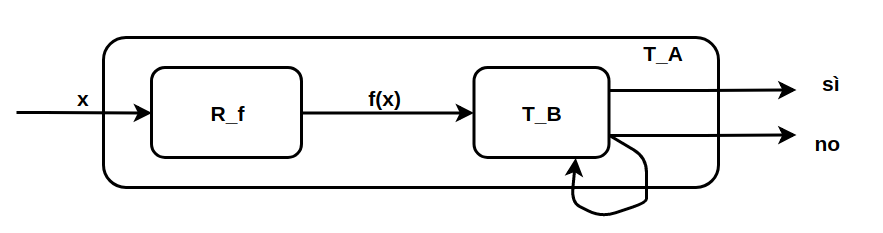
\includegraphics[scale=0.5]{teorema-1}
\end{figure}

\subparagraph{Corollario} $A \ \neg \text{Turing-riconoscibile e } A \leq_m B \implies B \ \neg \text{Turing-riconoscibile}$

\paragraph{Teorema}
\[
	A \leq_m B \iff \neg A \leq_m \neg B
\]
\subparagraph{Prova} Se $A \leq_m B$ allora deve esistere una qualche $f$ di riduzione per cui $\forall a \in A, \ b \in B \quad a \xmapsto{f} b$ (istanze sì) e $\forall x \notin A, \ y \notin B \quad x \xmapsto{f} y$ (istanze no).

Ma poiché le istanze sì di $\neg A$ sono le istanze no di $A$, e lo stesso vale per $B$, allora la $f$ è una funzione di riduzione anche per $\neg A$ e $\neg B$, in quanto:
\begin{enumerate}
 \item è ancora definita come $f: \Sigma^{\star} \to \Sigma^{\star}$
 \item è ancora calcolabile
 \item mappa ancora istanze sì ad istanze sì e istanze no ad istanze no
 \end{enumerate}
Abbiamo quindi esibito una funzione di riduzione di $\neg A$ a $\neg B$, perciò possiamo scrivere $\neg A \leq_m \neg B$.

Naturalmente per dimostrare l'altro verso della implicazione basta prendere $A' = \neg A$ e $B' = \neg B$ e applicare l'implicazione dimostrata precedentemente: \\
$A' \leq_m B' \implies \neg A' \leq_m \neg B'$ che è come dire $\neg A \leq_m \neg B \implies A \leq_m B$.

Quindi è vera la coimplicazione.

\subsection{Il problema dell'equivalenza $EQ_{TM}$}

Le istanze sì del problema sono costituite da tutte le codifiche di una coppia di macchine di Turing $T_1, T_2$\textit{equivalenti}, ovvero tali che $L(T_1) = L(T_2)$. 

\[
	EQ_{TM} = \{ <T_1, T_2> \ | \ T_1, T_2 \in TM \land L(T_1) = L(T_2)  \}
\]

Questo problema non solo è indecidibile, ma è anche non Turing-riconoscibile. Inoltre è l'unico problema che incontriamo nel corso per cui anche il complemento è non Turing-riconoscibile

\paragraph{Teorema} $EQ_{TM}$, il problema dell'equivalenza tra $TM$, non è Turing-riconoscibile

\subparagraph{Prova} Riduciamo $\neg A_{TM}$, che sappiamo essere non Turing-riconoscibile, a $EQ_{TM}$:
\[
	\neg A_{TM} \leq_m EQ_{TM}
\]
Tuttavia ridurre \textit{da} un problema non Turing-riconoscibile è complicato perché bisogna effettuare un mapping $<M, w> \xmapsto{f} <T_1, T_2>$che garantisce che $<T_1, T_2> \in L(EQ_{TM})$ non solo se $M$ rifiuta $w$, ma anche se $M$ non si ferma su $w$. Questa ultima condizione è chiaramente difficile da imporre.

Sfruttiamo allora il teorema di equivalenza tra riduzioni per portarci ad un caso più trattabile:
\[
	\neg A_{TM} \leq_m EQ_{TM} \text{ è come dire } A_{TM} \leq_m \neg EQ_{TM}
\]
Vogliamo quindi esibire una $f$ così definita:
\begin{gather*}
	f: \Sigma^{\star} \to \Sigma^{\star} \text{ calcolabile} \\
	<M, w> \xmapsto{f} <T_1, T_2> \text{ tale che } w \in L(M) \iff <T_1, T_2> \notin EQ_{TM}
\end{gather*}

L'idea è quindi fare sì che le $T_1, T_2$ costruite riconoscano lo stesso linguaggio se $w \notin L(M)$, mentre riconoscano due linguaggi diversi se $w \in L(M)$. Il modo più semplice di farlo è costruire $T_1$ in modo che non accetta mai nulla, ovvero tale che $L(T_1) = \varnothing$ sempre, mentre $T_2$ nel seguente modo:
\[
	\begin{cases}
		w \in L(M) \implies T_2 \text{ accetta qualsiasi x, ovvero } L(T_2) = \Sigma^{\star} \\
		w \notin L(M) \implies T_2 \text{ non accetta alcun x, ovvero } L(T_2) = \varnothing
	\end{cases}
\]
Quindi una $R_f$ che calcola $f$ ad alto livello è così definita:

\begin{description}
\item \textit{input}: $<M, w>$
\item \textit{output}: $<T_1, T_2>$ così definite:
\begin{itemize}
\item $T_1$:
\begin{description}
	\item \textit{input}: $x$
	\item \textit{descrizione}:
	\begin{enumerate}
	\item rifiuta $x$
	\end{enumerate}
\end{description}

\vspace{1cm}

\item $T_2$
\begin{description}
\item \textit{input}: $x$

\item \textit{descrizione}:
\begin{enumerate}
\item esegui $M$ su $w$
\item se $M$ accetta $w$ allora accetta $x$
\item se $M$ rifiuta $w$ allora rifiuta $x$
\end{enumerate}
\end{description}
\end{itemize}
\end{description}

\subparagraph{Prova di correttezza}

Vediamo se $R_f$ così costruita rispetta la proprietà voluta:

\begin{itemize}
\item se $M$ accetta $w$, allora $L(T_1) = \varnothing$ mentre $T_2$ accetta qualsiasi $x$, per cui $L(T_2) = \Sigma^{\star}$, di conseguenza $L(T_1) \neq L(T_2) \implies <T_1, T_2> \notin EQ_{TM}$.

\item se $M$ \textit{non} accetta $w$, allora abbiamo due casi:
\begin{enumerate}
\item se $M$ rifiuta $w$, allora di nuovo $L(T_1) = \varnothing$, ma $T_2$ rifiuta qualsiasi $x$, per cui anche $L(T_2) = \varnothing$, di conseguenza $L(T_1) = L(T_2) \implies <T_1, T_2> \in EQ_{TM}$

\item se $M$ non si ferma su $w$, allora di nuovo $L(T_1) = \varnothing$, ma $T_2$ che esegue $M$ su $w$ a maggior ragione non si ferma, su nessun $x$, per cui anche $L(T_2) = \varnothing$, di conseguenza $L(T_1) = L(T_2) \implies <T_1, T_2> \in EQ_{TM}$
\end{enumerate}
Quindi in entrambi i casi la conseguenza è che $<T_1, T_2> \in EQ_{TM}$.
\end{itemize}

\paragraph{Teorema} Anche $\neg EQ_{TM}$ è non Turing-riconoscibile

\subparagraph{Prova} Come prima riduciamo $\neg A_{TM}$, che sappiamo essere non Turing-riconoscibile, a $\neg EQ_{TM}$:
\[
	\neg A_{TM} \leq_m \neg EQ_{TM}
\]

Di nuovo sfruttiamo il teorema di equivalenza tra riduzioni per portarci ad un caso più trattabile:
\[
	\neg A_{TM} \leq_m \neg EQ_{TM} \text{ è come dire } A_{TM} \leq_m EQ_{TM}
\]
Vogliamo quindi esibire una $f$ così definita:
\begin{gather*}
	f: \Sigma^{\star} \to \Sigma^{\star} \text{ calcolabile} \\
	<M, w> \xmapsto{f} <T_1, T_2> \text{ tale che } w \in L(M) \iff <T_1, T_2> \in EQ_{TM}
\end{gather*}

L'idea è esattamente la stessa della prova del teorema precedente, ma cambia come costruiamo $T_1$ e $T_2$. $T_1$ invece di non accettare alcun $x$, accetta ogni $x$, quindi $L(T_1) = \Sigma^{\star}$; $T_2$ invece è identico al $T_2$ precedente:
\[
	\begin{cases}
		w \in L(M) \implies T_2 \text{ accetta qualsiasi x, ovvero } L(T_2) = \Sigma^{\star} \\
		w \in L(M) \implies T_2 \text{ non accetta alcun x, ovvero } L(T_2) = \varnothing
	\end{cases}
\]
Quindi una $R_f$ che calcola $f$ ad alto livello è così definita:

\begin{description}
\item \textit{input}: $<M, w>$
\item \textit{output}: $<T_1, T_2>$ così definite:
\begin{itemize}
\item $T_1$:
\begin{description}
	\item \textit{input}: $x$
	\item \textit{descrizione}:
	\begin{enumerate}
	\item accetta $x$
	\end{enumerate}
\end{description}

\item $T_2$
\begin{description}
\item \textit{input}: $x$

\item \textit{descrizione}:
\begin{enumerate}
\item esegui $M$ su $w$
\item se $M$ accetta $w$ allora accetta $x$
\item se $M$ rifiuta $w$ allora rifiuta $x$
\end{enumerate}
\end{description}
\end{itemize}
\end{description}

\subparagraph{Prova di correttezza}

Vediamo se $R_f$ così costruita rispetta la proprietà voluta:

\begin{itemize}
\item se $M$ accetta $w$, allora $L(T_1) = \Sigma^{\star}$ e $T_2$ accetta qualsiasi $x$, per cui $L(T_2) = \Sigma^{\star}$, di conseguenza $L(T_1) = L(T_2) \implies <T_1, T_2> \in EQ_{TM}$.

\item se $M$ \textit{non} accetta $w$, allora abbiamo due casi:
\begin{enumerate}
\item se $M$ rifiuta $w$, allora di nuovo $L(T_1) = \Sigma^{\star}$, ma $T_2$ rifiuta qualsiasi $x$, per cui $L(T_2) = \varnothing$, di conseguenza $L(T_1) \neq L(T_2) \implies <T_1, T_2> \notin EQ_{TM}$

\item se $M$ non si ferma su $w$, allora di nuovo $L(T_1) = \Sigma^{\star}$, ma $T_2$ che esegue $M$ su $w$ a maggior ragione non si ferma, su nessun $x$, per cui $L(T_2) = \varnothing$, di conseguenza $L(T_1) \neq L(T_2) \implies <T_1, T_2> \notin EQ_{TM}$
\end{enumerate}
Quindi in entrambi i casi la conseguenza è che $<T_1, T_2> \notin EQ_{TM}$.
\end{itemize}

\subsection{Chiusura delle classi}

Ci chiediamo ora se le classi di linguaggi Turing-decidibili ($L(TM_d)$) e Turing-riconoscibili ($L(TM_r)$) sono chiuse rispetto alle operazioni di unione, intersezione e complemento. 

Prenderemo di volta in volta come esempio due $T_1, T_2 \in TM_d$ oppure $T_1, T_2 \in TM_r$ generiche che decidono o riconoscono due linguaggi generici $L_1, L_2$.

\paragraph{Unione}
\begin{itemize}

\item  $L(TM_d)$ Sì\\
Poiché $T_1, T_2$ sono entrambi decisori, entrambi si fermano sia in accettazione che in non accettazione. Quindi possiamo costruire una $T \in TM_d$ che accetta $L(T_1) \cup L(T_2)$:
\\
\begin{description}
	\item \textit{input}: $x$
	\item \textit{descrizione}:
	\begin{enumerate}
	\item esegue $T_1$ su $x$
	\item se $T_1$ accetta, allora accetta
	
	\item altrimenti esegue $T_2$ su $x$
	\item se $T_2$ accetta, allora accetta
	
	\item altrimenti rifiuta
	\end{enumerate}
\end{description}

\item $L(TM_r)$ Sì\\
Poiché $T_1, T_2$ \textit{non} sono decisori, non possiamo semplicemente eseguirli in sequenza, perché una parola accettata da $T_2$ potrebbe non venire accettata dalla "macchina unione" se $T_1$ non termina su di essa. Quindi le due macchine verranno eseguite "in parallelo", ovvero un passo di calcolo alla volta, su due nastri diversi della macchina unione $T$:
\begin{description}
	\item \textit{input}: $x$
	\item \textit{descrizione}:
	\begin{enumerate}
	\item copia l'input sul secondo nastro
	\item esegui un passo di calcolo di $T_1$ sul primo nastro
	\item se $T_1$ raggiunge una configurazione di accettazione, allora accetta (e termina)
	\item altrimenti esegui un passo di calcolo di $T_2$ sul secondo nastro
	\item se $T_2$ raggiunge una configurazione di accettazione, allora accetta (e termina)
	
	\item torna al punto 2
	\end{enumerate}
\end{description}

\end{itemize}

\paragraph{Intersezione}
\begin{itemize}

\item $L(TM_d)$ Sì \\
Eseguiamo $T_1, T_2$ in sequenza, sapendo che entrambi si fermeranno su qualsiasi input:
\begin{description}
	\item \textit{input}: $x$
	\item \textit{descrizione}:
	\begin{enumerate}
	\item esegue $T_1$ su $x$
	\item se $T_1$ rifiuta, allora rifiuta (e termina)
	\item altrimenti esegue $T_2$ su $x$
	\item se $T_2$ accetta, allora accetta
	\item se $T_2$ rifiuta, allora rifiuta
	\end{enumerate}
\end{description}

\item $L(TM_r)$ Sì \\
Possiamo eseguire le due macchine $T_1, T_2$ semplicemente in sequenza, in quanto se anche una delle due non terminasse su qualche input $x$, allora $x$ non sarebbe nel suo linguaggio e quindi nemmeno nell'intersezione dei due:
\begin{description}
	\item \textit{input}: $x$
	\item \textit{descrizione}:
	\begin{enumerate}
	\item esegue $T_1$ su $x$
	\item se $T_1$ rifiuta, allora rifiuta (e termina)
	\item altrimenti esegue $T_2$ su $x$
	\item se $T_2$ accetta, allora accetta
	\item se $T_2$ rifiuta, allora rifiuta
	\end{enumerate}
\end{description}

\end{itemize}

\paragraph{Complemento}
\begin{itemize}
\item $L(TM_d)$ Sì \\
Basta costruire una macchina $\overline{T} \in TM_d$ che "inverte le uscite" di $T \in TM_d$:
\begin{description}
	\item \textit{input}: $x$
	\item \textit{descrizione}:
	\begin{enumerate}
	\item esegue $T$ su $x$
	\item se $T$ accetta, allora rifiuta
	\item se $T$ rifiuta, allora accetta
	\end{enumerate}
\end{description}

\item $L(TM_r)$ No \\
Se $T \in TM_r$ riconosce un certo $L$, allora in $\overline{L}$ ci devono essere sia le parole che $T$ rifiuta ma anche quelle su cui $T$ non termina. Ma si è dimostrato che data una $TM$ e un suo input, non siamo in grado di stabilire se questa termini oppure no, quindi non siamo in grado di individuare alcune delle parole che dovrebbero stare in $\overline{L}$, quindi non possiamo costruire un $\overline{T} \in TM_r$ che lo riconosce. 

\end{itemize}

\subsection{Ulteriore esercizio su riduzione}

\[
	PART = \{ <T> \ | \ T \in TM \land 010 \in L(T) \} \text{ è non decidibile}
\]

Per mostrarne la non decidibilità riduciamo, come sempre, $A_{TM}$ ad esso: $A_{TM} \leq_m PART$. Questo implica costruire una macchina $R_f$ che calcola una $f$ così definita:
\[
	<M, w> \xmapsto{f} <T> \text{ tale che } w \in L(M) \iff 010 \in L(T)
\]
Come spesso facciamo, ci poniamo nel caso più semplice, ovvero scegliamo come $L(T)$ che rispetterà la condizione il singoletto $\{ 010 \}$ (potremmo anche equivalentemente scegliere $\Sigma^{\star}$, in quanto $010 \in \Sigma^{\star}$), mentre scegliamo come $L(T)$ che \textit{non} rispetterà la condizione il linguaggio vuoto.

Quindi quando $M$ accetta $w$ la macchina $T$ costruita da $R_f$ accetterà solo input $x = 010$, mentre quando $M$ \textit{non} accetta $w$ la macchina $T$ non accetterà alcun $x$.

Una $R_f$ che calcola $f$ ad alto livello è così definita:

\begin{description}
\item \textit{input}: $<M, w>$
\item \textit{output}: $<T>$ così definita:
\begin{description}
	\item \textit{input}: $x$
	\item \textit{descrizione}:
	\begin{enumerate}
	\item se $x \neq 010$, allora rifiuta $x$ (non necessario se associamo $L(T) = \Sigma^{\star}$ alla istanza sì di $A_{TM}$)
	\item esegui $M$ su $w$
	\item se $M$ accetta $w$, allora accetta $x$
	\item se $M$ rifiuta $w$, allora rifiuta $x$
	\end{enumerate}
\end{description}
\end{description}

\subparagraph{Prova di correttezza}

Vediamo se $R_f$ così costruita rispetta la proprietà voluta:

\begin{itemize}
\item Se $M$ accetta $w$, allora $L(T) = \{010\}$ (oppure $\Sigma^{\star}$) ed evidentemente $010 \in L(T)$.

\item se $M$ \textit{non} accetta $w$, allora abbiamo due casi:
\begin{enumerate}
\item se $M$ rifiuta $w$, allora $L(T) = \varnothing$ ed evidentemente $010 \notin L(T)$

\item se $M$ non si ferma su $w$, allora $T$ che esegue $M$ su $w$ a maggior ragione non si ferma, su nessun $x$, per cui $L(T_2) = \varnothing$, di conseguenza di nuovo $L(T) = \varnothing$ ed evidentemente $010 \notin L(T)$
\end{enumerate}
Quindi in entrambi i casi la conseguenza è che $010 \notin L(T)$.
\end{itemize}